\section{Critério das áreas iguais}
\begin{frame}
\frametitle{Relação entre o ângulo de potência}
\begin{figure}[H]
\begin{flushright}
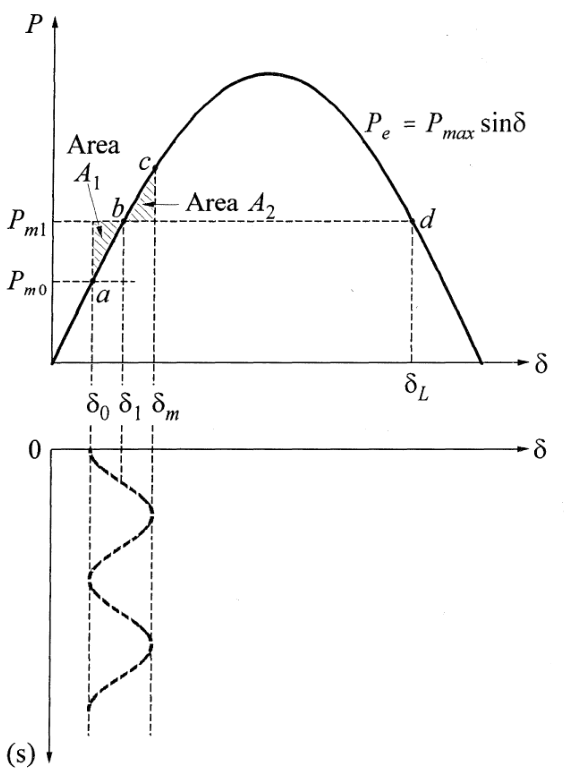
\includegraphics[width=5cm]{imagens/maq5.png}  
\end{flushright}
%\caption{Resultado prático da planta em malha aberta.}
\label{maq5} 
\end{figure}


\begin{textblock*}{10pt}(20pt,50pt)
\small
\begin{equation*}
   \frac{d^{2} \delta}{d t^2} = \frac{\omega_0}{2H}(P_m-P_e)
\end{equation*}
\vspace{0.5pt}
\begin{equation*}
   2\frac{d \delta}{d t}\frac{d^{2} \delta}{d t^2} = \frac{\omega_0(P_m-P_e)}{H}\frac{d \delta}{d t}
\end{equation*}
\vspace{0.5pt}
\begin{equation*}
   \frac{d}{d t}\left(\frac{d^{2} \delta}{d t^2}\right)^2 = \frac{\omega_0(P_m-P_e)}{H}\frac{d \delta}{d t}
\end{equation*}
\vspace{0.5pt}
\begin{equation*}
   \left(\frac{d^{2} \delta}{d t^2}\right)^2 =\int \frac{\omega_0(P_m-P_e)}{H}d \delta
\end{equation*}
\end{textblock*}


\begin{textblock*}{10pt}(170pt,70pt)
\small
\begin{equation*}
   \int_{\delta_0}^{\delta_m} \frac{\omega_0(P_m-P_e)}{H}d \delta = 0
\end{equation*}
\vspace{0.5pt}
\begin{equation*}
   E_1 = \int_{\delta_0}^{\delta_1} (P_m-P_e)d \delta = A_1
\end{equation*}
\vspace{0.5pt}
\begin{equation*}
   E_2 = \int_{\delta_1}^{\delta_m} (P_m-P_e)d \delta = A_2
\end{equation*}

\end{textblock*}

\end{frame}